\documentclass[journal,12pt,twocolumn]{IEEEtran}

\usepackage{setspace}
\usepackage{gensymb}

\singlespacing


\usepackage[cmex10]{amsmath}

\usepackage{amsthm}

\usepackage{mathrsfs}
\usepackage{txfonts}
\usepackage{stfloats}
\usepackage{bm}
\usepackage{cite}
\usepackage{cases}
\usepackage{subfig}

\usepackage{longtable}
\usepackage{multirow}

\usepackage{enumitem}
\usepackage{mathtools}
\usepackage{steinmetz}
\usepackage{tikz}
\usepackage{circuitikz}
\usepackage{verbatim}
\usepackage{tfrupee}
\usepackage[breaklinks=true]{hyperref}
\usepackage{graphicx}
\usepackage{tkz-euclide}
\usepackage{float}

\usetikzlibrary{calc,math}
\usepackage{listings}
    \usepackage{color}                                            %%
    \usepackage{array}                                            %%
    \usepackage{longtable}                                        %%
    \usepackage{calc}                                             %%
    \usepackage{multirow}                                         %%
    \usepackage{hhline}                                           %%
    \usepackage{ifthen}                                           %%
    \usepackage{lscape}     
\usepackage{multicol}
\usepackage{chngcntr}

\DeclareMathOperator*{\Res}{Res}

\renewcommand\thesection{\arabic{section}}
\renewcommand\thesubsection{\thesection.\arabic{subsection}}
\renewcommand\thesubsubsection{\thesubsection.\arabic{subsubsection}}

\renewcommand\thesectiondis{\arabic{section}}
\renewcommand\thesubsectiondis{\thesectiondis.\arabic{subsection}}
\renewcommand\thesubsubsectiondis{\thesubsectiondis.\arabic{subsubsection}}


\hyphenation{op-tical net-works semi-conduc-tor}
\def\inputGnumericTable{}                                 %%

\lstset{
%language=C,
frame=single, 
breaklines=true,
columns=fullflexible
}
\begin{document}
\newtheorem{theorem}{Theorem}[section]
\newtheorem{problem}{Problem}
\newtheorem{proposition}{Proposition}[section]
\newtheorem{lemma}{Lemma}[section]
\newtheorem{corollary}[theorem]{Corollary}
\newtheorem{example}{Example}[section]
\newtheorem{definition}[problem]{Definition}

\newcommand{\BEQA}{\begin{eqnarray}}
\newcommand{\EEQA}{\end{eqnarray}}
\newcommand{\define}{\stackrel{\triangle}{=}}
\bibliographystyle{IEEEtran}
\providecommand{\mbf}{\mathbf}
\providecommand{\pr}[1]{\ensuremath{\Pr\left(#1\right)}}
\providecommand{\qfunc}[1]{\ensuremath{Q\left(#1\right)}}
\providecommand{\sbrak}[1]{\ensuremath{{}\left[#1\right]}}
\providecommand{\lsbrak}[1]{\ensuremath{{}\left[#1\right.}}
\providecommand{\rsbrak}[1]{\ensuremath{{}\left.#1\right]}}
\providecommand{\brak}[1]{\ensuremath{\left(#1\right)}}
\providecommand{\lbrak}[1]{\ensuremath{\left(#1\right.}}
\providecommand{\rbrak}[1]{\ensuremath{\left.#1\right)}}
\providecommand{\cbrak}[1]{\ensuremath{\left\{#1\right\}}}
\providecommand{\lcbrak}[1]{\ensuremath{\left\{#1\right.}}
\providecommand{\rcbrak}[1]{\ensuremath{\left.#1\right\}}}
\theoremstyle{remark}
\newtheorem{rem}{Remark}
\newcommand{\sgn}{\mathop{\mathrm{sgn}}}
\providecommand{\abs}[1]{\vert#1\vert}
\providecommand{\res}[1]{\Res\displaylimits_{#1}} 
\providecommand{\norm}[1]{\lVert#1\rVert}
%\providecommand{\norm}[1]{\lVert#1\rVert}
\providecommand{\mtx}[1]{\mathbf{#1}}
\providecommand{\mean}[1]{E[ #1 ]}
\providecommand{\fourier}{\overset{\mathcal{F}}{ \rightleftharpoons}}
%\providecommand{\hilbert}{\overset{\mathcal{H}}{ \rightleftharpoons}}
\providecommand{\system}{\overset{\mathcal{H}}{ \longleftrightarrow}}
	%\newcommand{\solution}[2]{\textbf{Solution:}{#1}}
\newcommand{\solution}{\noindent \textbf{Solution: }}
\newcommand{\cosec}{\,\text{cosec}\,}
\providecommand{\dec}[2]{\ensuremath{\overset{#1}{\underset{#2}{\gtrless}}}}
\newcommand{\myvec}[1]{\ensuremath{\begin{pmatrix}#1\end{pmatrix}}}
\newcommand{\mydet}[1]{\ensuremath{\begin{vmatrix}#1\end{vmatrix}}}
\numberwithin{equation}{subsection}
\makeatletter
\@addtoreset{figure}{problem}
\makeatother
\let\StandardTheFigure\thefigure
\let\vec\mathbf
\renewcommand{\thefigure}{\theproblem}
\def\putbox#1#2#3{\makebox[0in][l]{\makebox[#1][l]{}\raisebox{\baselineskip}[0in][0in]{\raisebox{#2}[0in][0in]{#3}}}}
     \def\rightbox#1{\makebox[0in][r]{#1}}
     \def\centbox#1{\makebox[0in]{#1}}
     \def\topbox#1{\raisebox{-\baselineskip}[0in][0in]{#1}}
     \def\midbox#1{\raisebox{-0.5\baselineskip}[0in][0in]{#1}}
\vspace{3cm}
\title{GATE ASSIGNMENT 3}
\author{Dishank Jain \\ AI20BTECH11011}
\maketitle
\newpage
\bigskip
\renewcommand{\thefigure}{\theenumi}
\renewcommand{\thetable}{\theenumi}
Download all python codes from 
%
\begin{lstlisting}
https://github.com/Dishank422/EE3900/blob/main/Gate-Assignment3/codes
\end{lstlisting}
%
and latex-tikz codes from
%
\begin{lstlisting}
https://github.com/Dishank422/EE3900/blob/main/Gate-Assignment3/latex_code.tex
\end{lstlisting}
%
\section{EC 2005 Q.6}
The region of convergence of Z-transform of the sequence $\left(\dfrac{5}{6}\right)^nu(n) -\left(\dfrac{6}{5}\right)^nu(-n-1)$ must be
\begin{enumerate}[label = (\Alph*)]
\setlength\itemsep{0.7em}
    \item $\abs{Z} < \dfrac{5}{6}$
    \item $\abs{Z} > \dfrac{6}{5}$
    \item $\dfrac{5}{6} < \abs{Z} < \dfrac{6}{5}$
    \item $\dfrac{6}{5} < \abs{Z} < \infty$
\end{enumerate}

\section{Solution}
\begin{lemma}
The Z-transform of the sequence $a^nu(n)$ is $\dfrac{1}{1-az^{-1}}$ with a region of convergence $\abs{z} > \abs{a}$.
\end{lemma}
\begin{proof}
\begin{equation}
    \mathcal{Z}(a^nu(n)) = \sum_{n=0}^{\infty}a^nz^{-n} = \dfrac{1}{1-az^{-1}}
\end{equation}
ROC is given by $\abs{\dfrac{a}{z}} < 1$, i.e. $\abs{z} > \abs{a}$.
\end{proof}

\begin{lemma}
The Z-transform of the sequence $a^nu(-n)$ is $\dfrac{az^{-1}}{az^{-1}-1}$ with a region of convergence $\abs{z} < \abs{a}$.
\end{lemma}
\begin{proof}
\begin{equation}
    \mathcal{Z}(a^nu(-n)) = \sum_{n=-\infty}^{0}a^nz^{-n} = \sum_{n=0}^{\infty}a^{-n}z^{n} = \dfrac{az^{-1}}{az^{-1}-1}
\end{equation}
ROC is given by $\abs{\dfrac{z}{a}} < 1$, i.e. $\abs{z} < \abs{a}$.
\end{proof}
Therefore,
\begin{equation}
    \mathcal{Z}\left(\left(\dfrac{5}{6}\right)^nu(n)\right) = \dfrac{1}{1-\dfrac{5}{6}z^{-1}}
\end{equation}
with ROC $\abs{z} > \frac{5}{6}$. We shall call this ROC$_1$.

Moving ahead,
\begin{align}
    \mathcal{Z}\left(\left(\dfrac{6}{5}\right)^nu(-n-1)\right) &= z\left(\dfrac{6}{5}\right)^{-1}\mathcal{Z}\left(\left(\dfrac{6}{5}\right)^nu(-n)\right)\\
    &= \dfrac{1}{\dfrac{6}{5}z^{-1}-1}
\end{align}
with ROC $\abs{z} < \frac{6}{5}$. We shall call this ROC$_2$. The ROC of the given expression will be the intersection of ROC$_1$ and ROC$_2$. Therefore, the ROC of the given sequence is $\dfrac{5}{6} < \abs{z} < \dfrac{6}{5}$. Therefore, option (C) is the correct option.

The Z-transform of the given sequence is 
\begin{align}
&\dfrac{1}{1-\dfrac{5}{6}z^{-1}}+\dfrac{1}{1-\dfrac{6}{5}z^{-1}}\label{z}\\ 
= &\dfrac{2-\dfrac{61}{30}z^{-1}}{\left(1-\dfrac{5}{6}z^{-1}\right)\left(1-\dfrac{6}{5}z^{-1}\right)}
\end{align}
Therefore the poles of the Z-transform are given by 
\begin{equation}
    z = \dfrac{5}{6},\; \dfrac{6}{5}
\end{equation}
The zero of the Z-transform is given by 
\begin{equation}
    z = \dfrac{61}{60}
\end{equation}

\begin{lemma}
A system is causal if and only if the ROC of the Z-transform of the impulse response of the system lies outside the outermost pole.
\label{causility}
\end{lemma}

\begin{lemma}
A system is stable if and only if the ROC of the Z-tranform of the impulse response of the system includes the unit circle.
\label{stability}
\end{lemma}

Assuming that the given sequence is the impulse response of some system, then using lemmas \ref{causility} and \ref{stability}, the system is not causal but stable. The above two lemmas further result in lemma \ref{combo}.
\begin{lemma}
A causal system is stable if and only if all the poles of the Z-transform of the impulse response of the system lie inside the unit circle.
\label{combo}
\end{lemma}

\begin{figure}
    \centering
    \resizebox{\columnwidth}{!}{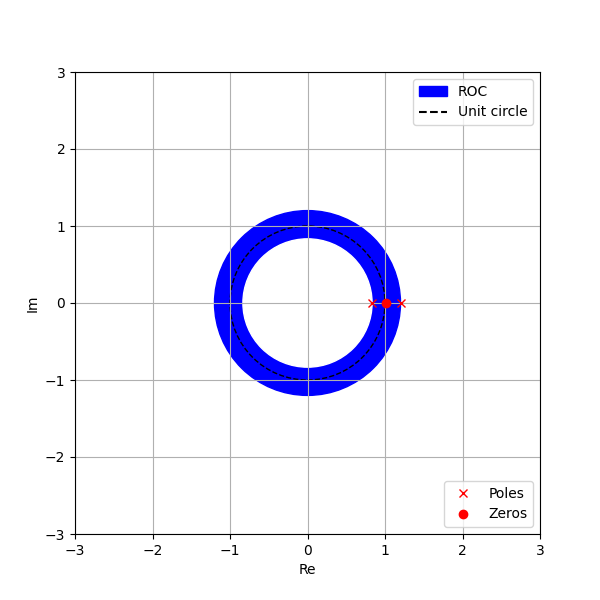
\includegraphics{figures/plot.png}}
    \caption{Pole-zero plot of the system}
    \label{plot}
\end{figure}

The DTFT of the sequence can be found by substituting $z = e^{j\omega}$ in \ref{z} as 
\begin{equation}
    \vec{H}(e^{j\omega}) = \dfrac{1}{1-\dfrac{5}{6}e^{-j\omega}}+\dfrac{1}{1-\dfrac{6}{5}e^{-j\omega}}
\end{equation}

The plot of magnitude of this DTFT is given in figure \ref{DTFT}. From this plot, we can observe that the given filter is a low-pass filter.
\begin{figure}
    \centering
    \resizebox{\columnwidth}{!}{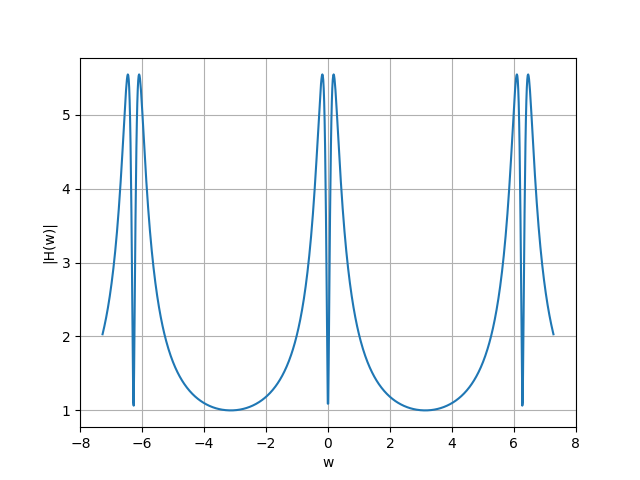
\includegraphics{figures/DTFT.png}}
    \caption{DTFT of the filter}
    \label{DTFT}
\end{figure}
\end{document}
